\documentclass[11pt]{article}
\usepackage[margin=1in]{geometry}
\usepackage{amsmath,amssymb}
\usepackage{tikz}
\usetikzlibrary{arrows.meta,positioning,shapes.geometric,calc,decorations.pathreplacing}
\usepackage{pgfplots}
\pgfplotsset{compat=1.18}
\usepackage[most]{tcolorbox}
\usepackage{booktabs}
\usepackage{listings}
\usepackage[colorlinks=true,linkcolor=blue!60!black]{hyperref}
\usepackage{xcolor}

\definecolor{ddpgblue}{RGB}{42,120,214}
\definecolor{dipred}{RGB}{190,40,40}
\definecolor{okgreen}{RGB}{20,130,60}
\definecolor{softgray}{RGB}{245,245,248}
\definecolor{codegray}{RGB}{248,248,245}

\lstset{
  language=Python, basicstyle=\ttfamily\small,
  keywordstyle=\color{ddpgblue}\bfseries,
  commentstyle=\color{okgreen}\itshape,
  stringstyle=\color{dipred},
  backgroundcolor=\color{codegray},
  frame=single, rulecolor=\color{black!25},
  breaklines=true, showstringspaces=false,
  numbers=left, numberstyle=\tiny\color{black!40}, numbersep=6pt
}

\newtcolorbox{ideabox}[1][]{colback=blue!4,colframe=ddpgblue,fonttitle=\bfseries,
  title={#1},breakable,enhanced}
\newtcolorbox{analogybox}{colback=green!5,colframe=okgreen,fonttitle=\bfseries,
  title={Everyday Analogy},breakable,enhanced}
\newtcolorbox{warnbox}[1][Key Problem]{colback=red!4,colframe=dipred,fonttitle=\bfseries,
  title={#1},breakable,enhanced}

\title{\textbf{Why Your DDPG Learning Curve Looks Like That}\\[2mm]
\large Plateau $\rightarrow$ Sudden Drop $\rightarrow$ Non-linear Rise $\rightarrow$ Stability:\\
A Complete Diagnosis of the Wiretap Power-Control Agent, with Fixes}
\author{}
\date{July 15, 2026}

\begin{document}
\maketitle
\vspace{-8mm}

\begin{center}
\begin{tcolorbox}[colback=softgray,colframe=black!40,width=0.92\textwidth]
\small \textbf{The question this document answers.} An ideal DDPG learning curve
starts low, rises non-linearly, and settles at a stable value. Your curve instead
\emph{starts} at an apparently stable level, \emph{drops} suddenly, \emph{then} rises
non-linearly and stabilizes. This document explains every phase of that shape using
your actual code (\texttt{ddpg.py} + \texttt{wiretap\_env.py}), gives worked numerical
examples, and provides the exact code fixes that recover the textbook curve.
\end{tcolorbox}
\end{center}

\tableofcontents

%====================================================================
\section{The Two Curves, Side by Side}

Let us first draw precisely what you expected and what you observed.

\begin{center}
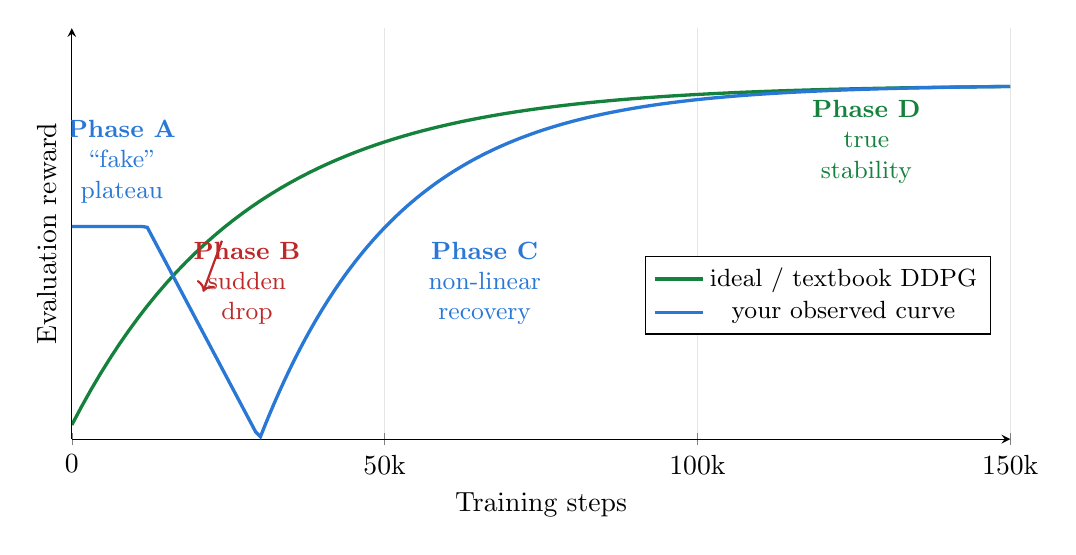
\begin{tikzpicture}
\begin{axis}[
  width=13.5cm, height=6.8cm,
  xlabel={Training steps}, ylabel={Evaluation reward},
  xmin=0, xmax=150, ymin=-0.2, ymax=1.25,
  xtick={0,50,100,150}, xticklabels={0, 50k, 100k, 150k},
  ytick=\empty,
  axis lines=left, grid=both, grid style={black!10},
  legend style={font=\small, at={(0.98,0.35)}, anchor=east}]
% ideal curve: monotone saturating
\addplot[very thick, okgreen, domain=0:150, samples=100]
   {1.05*(1-exp(-x/28)) - 0.15*exp(-x/28)};
\addlegendentry{ideal / textbook DDPG}
% observed: flat plateau, dip, recovery, plateau
\addplot[very thick, ddpgblue, samples=200, domain=0:150]
   { (x<12)*0.55
   + (x>=12)*(x<30)*(0.55 - 0.75*(x-12)/18)
   + (x>=30)*( -0.2 + 1.25*(1-exp(-(x-30)/22)) ) };
\addlegendentry{your observed curve}
% annotations
\node[font=\small, ddpgblue, align=center] at (axis cs:8,0.78)
  {\textbf{Phase A}\\ ``fake''\\ plateau};
\node[font=\small, dipred, align=center] at (axis cs:28,0.35)
  {\textbf{Phase B}\\ sudden\\ drop};
\node[font=\small, ddpgblue, align=center] at (axis cs:66,0.35)
  {\textbf{Phase C}\\ non-linear\\ recovery};
\node[font=\small, okgreen, align=center] at (axis cs:127,0.85)
  {\textbf{Phase D}\\ true\\ stability};
\draw[->, thick, dipred] (axis cs:24,0.5) -- (axis cs:21,0.32);
\end{axis}
\end{tikzpicture}
\end{center}

\begin{ideabox}[The one-sentence diagnosis]
Phase A is \emph{not} learned stability --- it is an \textbf{untrained constant
policy} that only \emph{looks} stable; Phase B is the actor being dragged downhill by
a \textbf{still-random critic}; Phases C--D are ordinary DDPG learning once the
critic finally becomes accurate. Your curve is a well-known DDPG
``failure-then-recovery'' transient, amplified by four specific properties of your
code.
\end{ideabox}

The rest of the document proves each claim, phase by phase, then gives the fixes.

%====================================================================
\section{Background: What DDPG Is Actually Doing}

DDPG trains \textbf{two} neural networks that play different roles:

\begin{center}
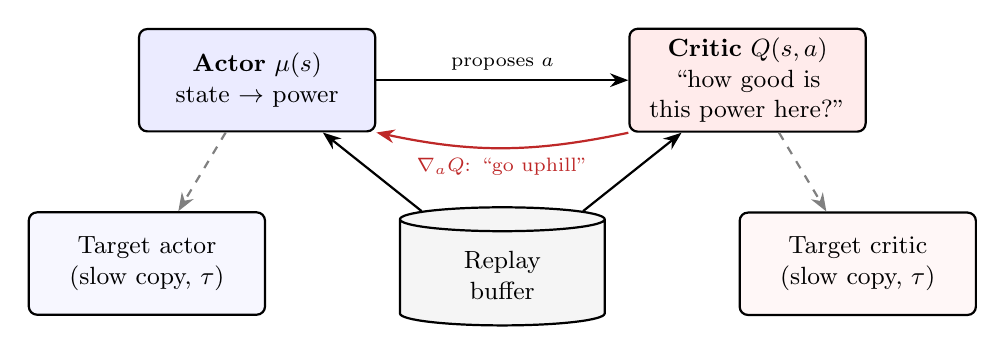
\begin{tikzpicture}[
  net/.style={draw, rounded corners=3pt, minimum width=30mm, minimum height=13mm,
              align=center, thick, font=\small},
  buf/.style={draw, cylinder, shape border rotate=90, aspect=0.25, minimum width=26mm,
              minimum height=15mm, align=center, thick, font=\small, fill=black!4},
  >=Stealth, node distance=14mm]
  \node[net, fill=blue!8]  (actor)  {\textbf{Actor} $\mu(s)$\\ state $\to$ power};
  \node[net, fill=red!8, right=32mm of actor] (critic) {\textbf{Critic} $Q(s,a)$\\ ``how good is\\ this power here?''};
  \node[buf, below=16mm of $(actor)!0.5!(critic)$] (buffer) {Replay\\ buffer};
  \node[net, fill=blue!3, below=10mm of actor, xshift=-14mm]  (actorT)  {Target actor\\ (slow copy, $\tau$)};
  \node[net, fill=red!3,  below=10mm of critic, xshift=14mm]  (criticT) {Target critic\\ (slow copy, $\tau$)};
  \draw[->, thick] (actor.east) -- node[above, font=\scriptsize]{proposes $a$} (critic.west);
  \draw[->, thick, dipred] (critic.south west) to[bend left=12]
        node[below, sloped, font=\scriptsize]{$\nabla_a Q$: ``go uphill''} (actor.south east);
  \draw[->, thick] (buffer) -- (actor);
  \draw[->, thick] (buffer) -- (critic);
  \draw[->, thick, black!50, dashed] (actor) -- (actorT);
  \draw[->, thick, black!50, dashed] (critic) -- (criticT);
\end{tikzpicture}
\end{center}

\begin{itemize}
\item The \textbf{critic} learns to predict the long-term reward $Q(s,a)$ of taking
      power $a$ in fading state $s$, by regression toward the bootstrapped target
      $r + \gamma\, Q_{\text{target}}(s', \mu_{\text{target}}(s'))$.
\item The \textbf{actor} never sees rewards directly. It is updated to \emph{climb
      the critic's landscape}: it moves its output in the direction the critic says
      is uphill.
\end{itemize}

\begin{analogybox}
The critic is a \textbf{map-maker} sketching a treasure map of the reward landscape;
the actor is a \textbf{hiker} who walks wherever the map says ``up.'' Early in
training the map is random scribbles --- and the hiker follows it anyway. That single
fact explains your sudden drop.
\end{analogybox}

%====================================================================
\section{Phase A: The ``Fake'' Plateau}

\subsection{A freshly initialized Sigmoid actor is a constant}

Your actor is \texttt{mlp([2,H,H,1], nn.Sigmoid)}. PyTorch initializes linear layers
with small weights centred on zero, so for \emph{any} input state the pre-activation
of the last layer is close to $0$, and
\[
\text{actor output} \;=\; \sigma(\text{pre-activation} \approx 0) \;\approx\; \sigma(0) = 0.5 .
\]

\begin{center}
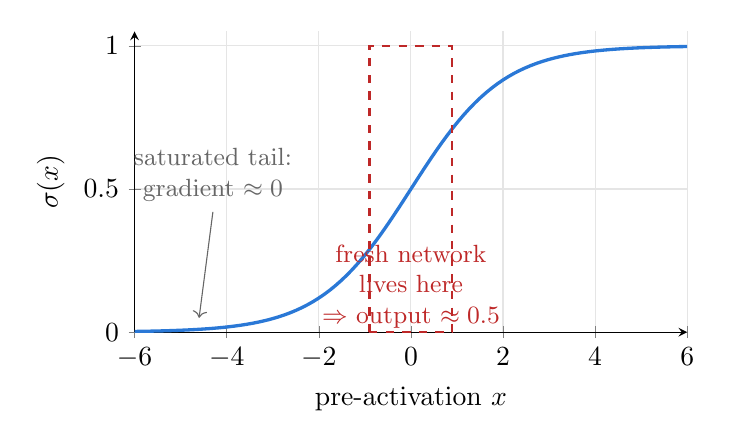
\begin{tikzpicture}
\begin{axis}[
  width=8.6cm, height=5.4cm,
  xlabel={pre-activation $x$}, ylabel={$\sigma(x)$},
  xmin=-6, xmax=6, ymin=0, ymax=1.05,
  axis lines=left, grid=both, grid style={black!10}]
  \addplot[very thick, ddpgblue, domain=-6:6, samples=100] {1/(1+exp(-x))};
  \draw[dashed, dipred, thick] (axis cs:-0.9,0) rectangle (axis cs:0.9,1.0);
  \node[font=\small, dipred, align=center] at (axis cs:0,0.16)
     {fresh network\\ lives here\\ $\Rightarrow$ output $\approx 0.5$};
  \node[font=\small, black!60, align=center] at (axis cs:-4.3,0.55)
     {saturated tail:\\ gradient $\approx 0$};
  \draw[->, black!60] (axis cs:-4.3,0.42) -- (axis cs:-4.6,0.05);
\end{axis}
\end{tikzpicture}
\end{center}

With your action mapping $P = P_{\min} + a\,(P_{\max}-P_{\min}) = 0.1 + a\cdot4.9$,
the untrained agent therefore plays a \textbf{constant power}
\[
P \approx 0.1 + 0.5 \times 4.9 = 2.55 \quad \text{in every state.}
\]

\subsection{Worked example: what reward does the constant policy earn?}

Take a mid-range fading state $\gamma_B=\gamma_E=1.6$ (middle of $[0.2,3]$), with your
constants $A_B=1.5$, $A_E=0.5$, $c_B=c_E=1$, $\lambda=0.3$, $\bar P=2$:
\[
v = \frac{1.6}{2.55}=0.627,\qquad
C_B=\log_2(1+1.5\cdot0.627)=0.958,\qquad
C_E=\log_2(1+0.5\cdot0.627)=0.395,
\]
\[
r = (0.958-0.395) - 0.3\,(2.55-2) = 0.563 - 0.165 = 0.398 .
\]
A perfectly ordinary, middling reward --- and here is the key point:

\begin{warnbox}[Why it looks stable when nothing has been learned]
A constant policy gives the \emph{same} average reward every time you evaluate it.
Your evaluation additionally \textbf{fixes the random seed to 42} at every
checkpoint, so even the fading sequences are identical across evaluations. Constant
policy $\times$ identical evaluation conditions $=$ a perfectly flat line that
\emph{mimics} convergence. Moreover, your first evaluation happens at step 5{,}000
--- you never plot the $t=0$ point, so the curve appears to ``begin'' at this false
plateau instead of at an untrained baseline.
\end{warnbox}

%====================================================================
\section{Phase B: The Sudden Drop --- Actor Follows a Garbage Critic}

\subsection{The mechanism}

Your training loop calls \texttt{agent.update()} from the very first step; updates
actually begin as soon as the buffer holds \texttt{BATCH = 128} samples --- i.e.\
after 128 steps of a 150{,}000-step run. At that moment:

\begin{enumerate}
\item The critic has seen only $\sim$128 transitions, all generated by one nearly
      constant policy (power $\approx 2.55$ plus small noise). Its $Q$-surface over
      the rest of the action range $[0.1, 5]$ is \textbf{unconstrained
      extrapolation} --- effectively random hills and valleys.
\item The actor is immediately trained to climb that random surface. Whatever
      direction the noise-hills point, the actor follows --- typically \emph{away}
      from its accidentally-reasonable constant $2.55$, into genuinely bad powers.
\item Real performance falls. The buffer then fills with low-reward data, the critic
      slowly corrects, and only later does the actor climb back.
\end{enumerate}

\begin{center}
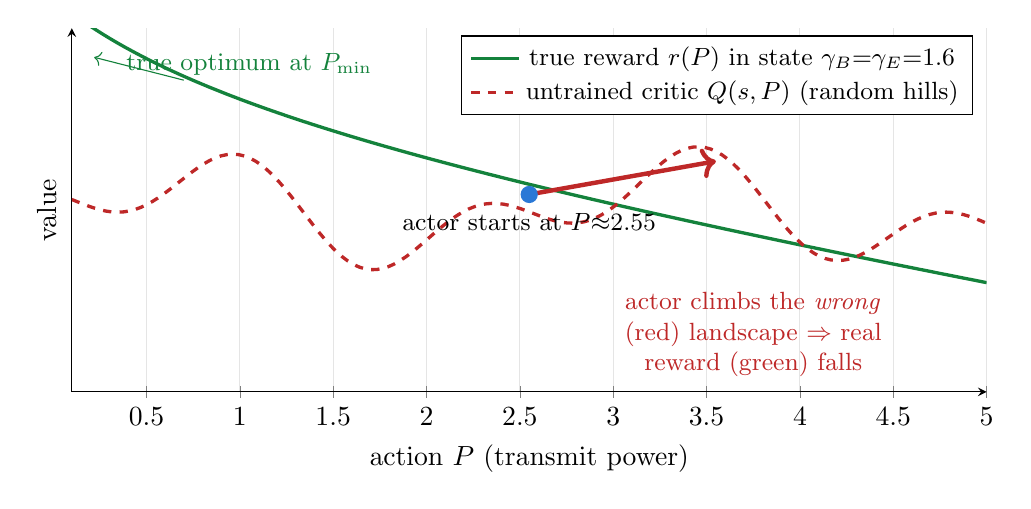
\begin{tikzpicture}
\begin{axis}[
  width=13.2cm, height=6.2cm,
  xlabel={action $P$ (transmit power)},
  ylabel={value},
  xmin=0.1, xmax=5, ymin=-1.6, ymax=1.9,
  ytick=\empty,
  axis lines=left, grid=both, grid style={black!10},
  legend style={font=\small, at={(0.985,0.98)}, anchor=north east}]
% true Q (monotone decreasing in P for this env)
\addplot[very thick, okgreen, domain=0.1:5, samples=120]
  {ln(1+1.5*1.6/x)/ln(2) - ln(1+0.5*1.6/x)/ln(2) - 0.3*(x-2)};
\addlegendentry{true reward $r(P)$ in state $\gamma_B{=}\gamma_E{=}1.6$}
% garbage critic
\addplot[very thick, dipred, dashed, domain=0.1:5, samples=160]
  {0.35*sin(deg(2.4*x))+0.3*cos(deg(5.1*x+1))+0.15};
\addlegendentry{untrained critic $Q(s,P)$ (random hills)}
% actor position and pull
\draw[->, ultra thick, dipred] (axis cs:2.55,0.30) -- (axis cs:3.55,0.62);
\node[circle, fill=ddpgblue, inner sep=2.2pt, label={[font=\small]below:{actor starts at $P{\approx}2.55$}}]
   at (axis cs:2.55,0.30) {};
\node[font=\small, dipred, align=center] at (axis cs:3.75,-1.05)
  {actor climbs the \emph{wrong}\\ (red) landscape $\Rightarrow$ real\\ reward (green) falls};
\node[font=\small, okgreen] at (axis cs:1.05,1.55) {true optimum at $P_{\min}$};
\draw[->, okgreen] (axis cs:0.7,1.4) -- (axis cs:0.22,1.62);
\end{axis}
\end{tikzpicture}
\end{center}

\begin{analogybox}
The hiker (actor) was standing, by pure luck, on a decent ledge. Then the map-maker
(critic) hands over the first draft of the map --- random scribbles --- and the hiker
\emph{obediently walks off the ledge}. That step off the ledge is your sudden drop.
Only after the map-maker has surveyed enough terrain does the map become truthful,
and the hiker climbs back up.
\end{analogybox}

\subsection{Three amplifiers specific to your code}

\begin{enumerate}
\item \textbf{No warm-up.} Standard practice fills the buffer with \emph{uniformly
      random} actions for several thousand steps before any gradient update, so the
      critic's first lessons cover the whole action range. Your critic's first
      lessons cover only a sliver around $P=2.55$.
\item \textbf{Needless bootstrapping ($\gamma=0.99$).} Look carefully at your
      environment: the AR(1) fading update
      \[
      \gamma_B' = \rho_B\gamma_B + (1-\rho_B)\,U, \qquad
      \gamma_E' = \rho_E\gamma_E + (1-\rho_E)\,U'
      \]
      \textbf{never involves the action $P$.} The action affects only the immediate
      reward, never the next state --- your problem is a \emph{contextual bandit},
      not a full MDP (see diagram below). With $\gamma=0.99$ the critic is forced to
      also predict the value of future fading it cannot influence; early
      bootstrapped targets $r+\gamma Q_{\text{target}}$ are then dominated by the
      (random) target-critic term, making the drop deeper and longer.
\item \textbf{Actor and critic learn at the same speed.} Both use
      $\text{LR}=3\times10^{-4}$ and update every step. The actor exploits critic
      errors as fast as they appear; delaying/slowing the actor (the central idea of
      TD3) damps exactly this transient.
\end{enumerate}

\begin{center}
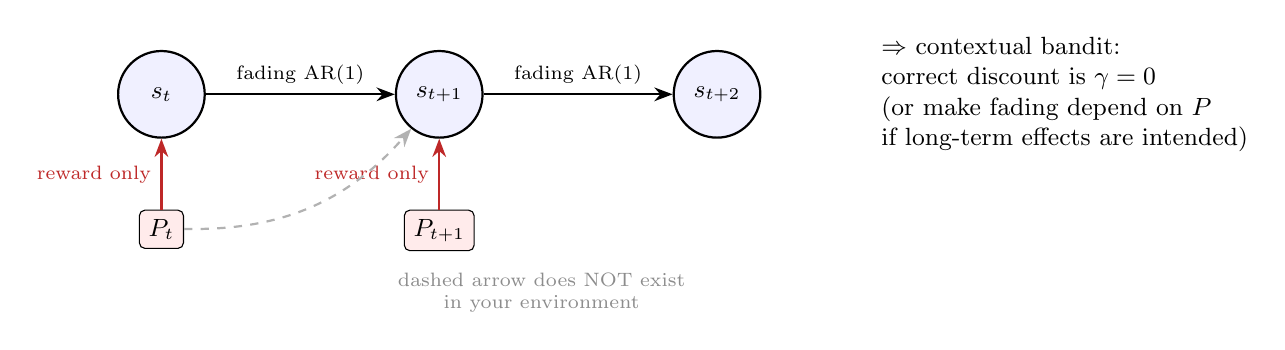
\begin{tikzpicture}[
  st/.style={draw, circle, minimum size=11mm, thick, font=\small, fill=blue!6},
  >=Stealth, node distance=24mm]
% MDP
\node[st] (s1) {$s_t$};
\node[st, right=of s1] (s2) {$s_{t+1}$};
\node[st, right=of s2] (s3) {$s_{t+2}$};
\draw[->, thick] (s1) -- node[above,font=\scriptsize]{fading AR(1)} (s2);
\draw[->, thick] (s2) -- node[above,font=\scriptsize]{fading AR(1)} (s3);
\node[draw, rounded corners=2pt, fill=red!8, below=9mm of s1, font=\small] (a1) {$P_t$};
\node[draw, rounded corners=2pt, fill=red!8, below=9mm of s2, font=\small] (a2) {$P_{t+1}$};
\draw[->, thick, dipred] (a1) -- node[left,font=\scriptsize]{reward only} (s1);
\draw[->, thick, dipred] (a2) -- node[left,font=\scriptsize]{reward only} (s2);
\draw[->, thick, black!30, dashed] (a1) to[bend right=25] (s2);
\node[font=\scriptsize, black!45, align=center, below=1.5mm of a2, xshift=13mm]
   {dashed arrow does NOT exist\\ in your environment};
\node[font=\small, align=left, right=14mm of s3]
  {$\Rightarrow$ contextual bandit:\\ correct discount is $\gamma=0$\\
   (or make fading depend on $P$\\ if long-term effects are intended)};
\end{tikzpicture}
\end{center}

%====================================================================
\section{Phases C and D: Recovery and (Real) Stability}

Once the buffer contains diverse experience --- including the bad powers visited
during the dip --- the critic's regression finally pins down the true shape of
$Q(s,P)$. The actor then climbs a \emph{truthful} landscape, and reward rises. The
rise is non-linear (fast at first, then saturating) for two stacked reasons:

\begin{enumerate}
\item \textbf{Diminishing distance to optimum.} Gradient ascent moves fastest when
      far from the peak and slows as it approaches --- the generic exponential-like
      saturation of learning curves.
\item \textbf{Sigmoid tail saturation.} In your environment the optimum is a
      \emph{corner}: with $P$ in the denominator of both $v_B$ and $v_E$, your own
      derivative
      \[
      \frac{\partial r}{\partial P}
      = \frac{1}{\ln 2}\left[\frac{t_E}{P^2+t_E P}-\frac{t_B}{P^2+t_B P}\right]-\lambda
      \;<\;0 \quad\text{whenever } t_B>t_E,
      \]
      so the best power is always $P_{\min}$ (exactly what the comment in your
      \texttt{waterfill\_P} says). To output $P_{\min}$ the actor's Sigmoid must
      saturate toward $0$ --- and in the Sigmoid tail the gradient
      $\sigma'(x)=\sigma(x)(1-\sigma(x))\to 0$, so the final approach crawls. That is
      the long flattening tail of Phase D.
\end{enumerate}

\begin{warnbox}[A modelling inconsistency worth fixing first]
Your plot title says $v = b^2\cdot P\cdot\gamma\cdot P_o$ (power in the
\textbf{numerator}) but the environment implements $v = \gamma P_o/(b^2 P)$ (power in
the \textbf{denominator}). These are different physical models with different optimal
policies: the numerator version has a genuine interior trade-off (more power $\to$
more secrecy but more penalty), giving a non-trivial water-filling baseline and an
actually interesting learning problem; the denominator version collapses to
``always transmit at $P_{\min}$.'' Decide which physics you mean \emph{before}
tuning the RL --- right now DDPG is spending 150k steps learning a corner solution.
\end{warnbox}

%====================================================================
\section{The Fixes, with Code}

Each fix targets one mechanism identified above.

\subsection{Fix 1: Random-action warm-up (kills the drop at its root)}

\begin{lstlisting}
WARMUP = 5000                      # steps of pure exploration
for t in range(1, steps + 1):
    if t <= WARMUP:
        P = np.random.uniform(env.P_min, env.P_max)   # uniform actions
    else:
        P = agent.act(s, noise_std=noise)
    s2, r, _, _ = env.step(P)
    agent.buf.push(s, P, r, s2); s = s2
    if t > WARMUP:                 # no gradient steps until buffer is diverse
        agent.update()
\end{lstlisting}

The critic's first lessons now cover the whole action range $[0.1,5]$, so its first
map already resembles the truth --- the hiker never walks off the ledge.

\subsection{Fix 2: Match the discount to the problem structure}

\begin{lstlisting}
GAMMA = 0.0    # contextual bandit: action never affects the next state
# critic target simplifies to:  q_tgt = R      (pure reward regression)
\end{lstlisting}

If you \emph{want} a genuine MDP (e.g.\ power choices heating the amplifier or
draining a battery, thereby affecting future states), add that coupling to
\texttt{step()} first --- then $\gamma=0.99$ earns its keep.

\subsection{Fix 3: Delayed, slower actor (the TD3 trick)}

\begin{lstlisting}
LR_ACTOR, LR_CRITIC = 1e-4, 3e-4
self.oa = torch.optim.Adam(self.actor.parameters(),  LR_ACTOR)
self.oc = torch.optim.Adam(self.critic.parameters(), LR_CRITIC)

def update(self):
    ...
    self.oc.zero_grad(); critic_loss.backward()
    torch.nn.utils.clip_grad_norm_(self.critic.parameters(), 1.0)
    self.oc.step()
    self.n_updates += 1
    if self.n_updates % 2 == 0:          # actor moves half as often
        self.oa.zero_grad(); actor_loss.backward()
        torch.nn.utils.clip_grad_norm_(self.actor.parameters(), 1.0)
        self.oa.step()
        soft(self.actor_t, self.actor); soft(self.critic_t, self.critic)
\end{lstlisting}

The map-maker now stays two steps ahead of the hiker.

\subsection{Fix 4: Evaluate at $t=0$ (honest curve start)}

\begin{lstlisting}
log.append((0, evaluate(lambda st: agent.act(st, 0.0), env, n_ep=eval_eps)))
\end{lstlisting}

Your curve will then visibly \emph{begin} at the untrained-constant-policy level,
and Phase A stops masquerading as convergence.

\subsection{Optional Fix 5: Escape the Sigmoid tail}

If the optimum stays at a corner ($P_{\min}$), replace the Sigmoid by
\texttt{nn.Tanh} mapped as $P = \bar m + \tfrac{a}{1}\cdot \tfrac{P_{\max}-P_{\min}}{2}$
with $\bar m = \tfrac{P_{\max}+P_{\min}}{2}$; Tanh also saturates, but its gradients
in the working region are $4\times$ larger, and corner actions are reached faster.
Alternatively keep Sigmoid and add a small action-space regularizer.

%====================================================================
\section{What the Curve Should Look Like After the Fixes}

\begin{center}
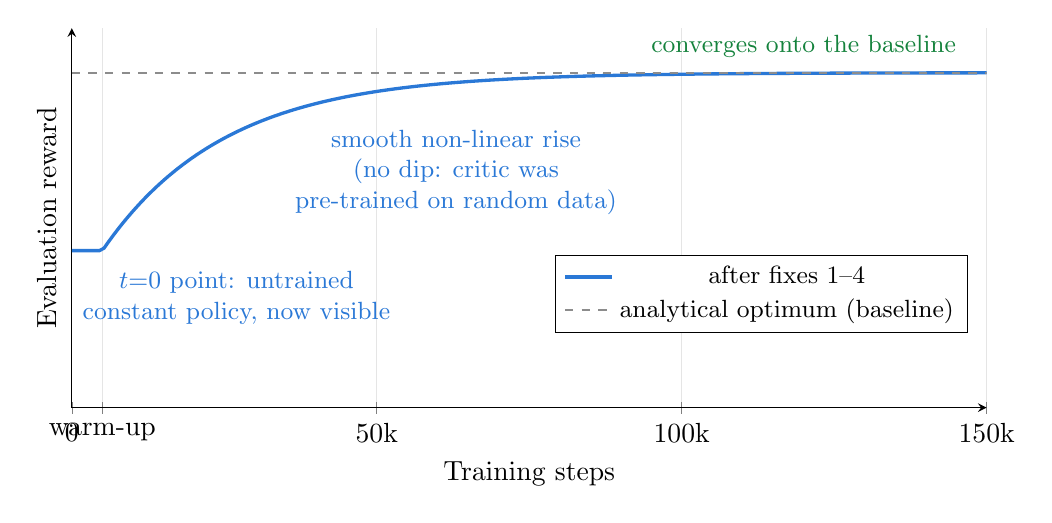
\begin{tikzpicture}
\begin{axis}[
  width=13.2cm, height=6.4cm,
  xlabel={Training steps}, ylabel={Evaluation reward},
  xmin=0, xmax=150, ymin=-0.2, ymax=1.25,
  xtick={0,5,50,100,150}, xticklabels={0, warm-up, 50k, 100k, 150k},
  ytick=\empty,
  axis lines=left, grid=both, grid style={black!10},
  legend style={font=\small, at={(0.98,0.30)}, anchor=east}]
\addplot[very thick, ddpgblue, samples=200, domain=0:150]
   { (x<5)*0.40 + (x>=5)*( 0.40 + 0.68*(1-exp(-(x-5)/20)) ) };
\addlegendentry{after fixes 1--4}
\addplot[thick, black!45, dashed, domain=0:150] {1.08};
\addlegendentry{analytical optimum (baseline)}
\node[font=\small, ddpgblue, align=center] at (axis cs:27,0.22)
  {$t{=}0$ point: untrained\\ constant policy, now visible};
\node[font=\small, ddpgblue, align=center] at (axis cs:63,0.70)
  {smooth non-linear rise\\ (no dip: critic was\\ pre-trained on random data)};
\node[font=\small, okgreen] at (axis cs:120,1.18) {converges onto the baseline};
\end{axis}
\end{tikzpicture}
\end{center}

\paragraph{Baseline caution.} With the current (denominator) physics, the correct
baseline is the constant policy $P_{\min}$, and your \texttt{waterfill\_P} already
returns it; after switching to the numerator physics, \texttt{waterfill\_P}'s
bisection on \texttt{dr\_dP} becomes a genuine interior water-filling solution and a
meaningful line to converge to.

%====================================================================
\section{Summary Table}

\begin{center}\small
\begin{tabular}{p{28mm}p{52mm}p{52mm}}
\toprule
\textbf{Curve phase} & \textbf{Root cause in your code} & \textbf{Fix}\\
\midrule
A. Initial ``stable'' plateau & Sigmoid init $\Rightarrow$ constant $P\approx2.55$;
fixed-seed eval makes it look converged; no $t{=}0$ point plotted &
Evaluate at $t=0$ (Fix 4); understand it is a baseline, not convergence\\[1mm]
B. Sudden drop & Actor climbs a random critic after only 128 samples; no warm-up;
$\gamma=0.99$ bootstraps noise; equal LRs & Warm-up (Fix 1); $\gamma=0$ (Fix 2);
delayed slower actor + grad clipping (Fix 3)\\[1mm]
C. Non-linear rise & Normal DDPG learning once critic is accurate & --- (expected)\\[1mm]
D. Final plateau & True optimum reached; slow tail from Sigmoid saturation at the
corner optimum $P_{\min}$ & Tanh head (Fix 5); or fix the physics so the optimum is
interior\\
\bottomrule
\end{tabular}
\end{center}

\begin{tcolorbox}[colback=softgray, colframe=black!40,
  title=\textbf{The whole diagnosis in four sentences}]
\begin{enumerate}
\item Your initial plateau is an untrained constant policy ($\sigma(0)=0.5 \Rightarrow
      P\approx2.55$) evaluated under a fixed seed --- fake stability.
\item The drop is the actor faithfully climbing a critic that is still random
      scribbles, made worse by no warm-up, needless $\gamma=0.99$ bootstrapping in
      what is really a contextual bandit, and equal actor/critic speeds.
\item The recovery and final plateau are ordinary DDPG convergence --- to a trivial
      corner optimum ($P_{\min}$), because your environment puts $P$ in the
      denominator while your plot title claims the numerator model.
\item Warm-up $+$ $\gamma=0$ $+$ delayed actor $+$ a $t{=}0$ evaluation point
      restores the textbook monotone curve; fixing the physics makes the problem
      worth learning.
\end{enumerate}
\end{tcolorbox}

\end{document}
